\documentclass[10pt,twocolumn,letterpaper]{article}

\usepackage{cvpr}
\usepackage{times}
\usepackage{epsfig}
\usepackage{graphicx}
\usepackage{amsmath}
\usepackage{amssymb}

% Include other packages here, before hyperref.

% If you comment hyperref and then uncomment it, you should delete
% egpaper.aux before re-running latex.  (Or just hit 'q' on the first latex
% run, let it finish, and you should be clear).
\usepackage[pagebackref=true,breaklinks=true,letterpaper=true,colorlinks,bookmarks=false]{hyperref}

% \cvprfinalcopy % *** Uncomment this line for the final submission

\def\cvprPaperID{****} % *** Enter the CVPR Paper ID here
\def\httilde{\mbox{\tt\raisebox{-.5ex}{\symbol{126}}}}

% Pages are numbered in submission mode, and unnumbered in camera-ready
\ifcvprfinal\pagestyle{empty}\fi
\begin{document}

%%%%%%%%% TITLE
\title{3D Reconstruction from Multi-View Stereo:\\ From Implementation to Oculus Virtual Reality}

\author{Andrew Moran\\
  MIT, \textit{Class of 2014}\\
  {\tt\small andrewmo@mit.edu}
% For a paper whose authors are all at the same institution,
% omit the following lines up until the closing ``}''.
% Additional authors and addresses can be added with ``\and'',
% just like the second author.
% To save space, use either the email address or home page, not both
\and
Ben Eysenbach\\
MIT\\
{\tt\small bce@mit.edu}
}

\maketitle
%\thispagestyle{empty}

%%%%%%%%% ABSTRACT
\begin{abstract}
   Multi-View Stereo reconstructs a 3D model from images. Each image is a projection of a 3D model onto the camera plane ($\mathbb{R}^3 \rightarrow \mathbb{R}^2$), which inherently results in a loss of information. With enough images taken from a variety of perspectives, an reasonable model of the original scene can be reconstructed. These reconstructions usually begin by determining where each image was taken from. Once the cameras are calibrated, a dense, colored point cloud can be generated. A mesh can be fit over the point cloud to represent structures in the original scene. This entire process can be visualized through an Oculus Rift.
\end{abstract}

%%%%%%%%% BODY TEXT
\section{Introduction}
Most current approaches to Multi-View Stereo can be broken down into three steps: feature matching, camera calibration, and dense reconstruction. In pipelines which result in a point cloud, surface reconstruction is applied as a final step.
%-------------------------------------------------------------------------
\subsection{Feature Matching}

The first step in most Multi-View Stereo pipelines is finding correspondence points between images. Once we know these points, we can determine the relative position of the cameras which took the images.

First, we select features of interest in each image. There exist numerous algorithms for selecting these points (SIFT, SURF). The general idea behind most of them is to find a feature which is unique enough such that finding a similar feature in another images indicates with high probability that the two features corresponds to the same object in the scene.\cite{brown}

Once features have been extracted from each image, pairwise matches must be found. Matches will not exist for all features, so some criteria must be specified for when to accept a match. One such criteria is to match two features if the first is the best match for the second, and the second is the best match for the first. Another approach is to match one feature to another feature if the second best match is a much worse match than the best match.\cite{brown}

\subsection{Camera Calibration}

Now that we have correspondence points, we want to compute a homography relating one image to another. If we only wanted to find the orientation of one camera relative to another, we could use RANSAC to fit a homography (with the Discrete Linear Transform to make it linear).\cite{ransac} However, if we only found the optimal pairwise relative positions, we would not be guaranteed that they would be consistent.

Instead, we want to find the \emph{global} optimal camera positions. This process is known as Sparse Bundle Adjustment, and can been seen as minimizing a series of nonlinear equations. The  Levenberg Marquardt Algorithm for nonlinear least-squares is commonly used as a subroutine. Sparse Bundler Adjustment incrementally alters the positions of the cameras to as to minimize the \emph{reprojective error} of the found correspondence points with respect to the images in which they appear. At the end of this process, we have a calibration matrix for each camera, relating the pose of each camera to a global coordinate system.\cite{snavely, sba}

\subsection{Dense Reconstruction}

We can now reconstruct the scene from calibrated cameras. We want to find eventually output a scene which is \emph{photo consistent}. Common approaches to this problem include: (1) building up a scene from points whose locations are found by triangulating between images; (2) starting with a volume which encloses the region of interest, and removing \emph{voxels} which are not photoconsistent; and (3) generating stereo depth maps for pairs of images, and then fusing them together.\cite{furukawa}

\begin{figure*}[t]
  \begin{center}
    %\fbox{\rule{0pt}{2in} \rule{0.9\linewidth}{0pt}}
    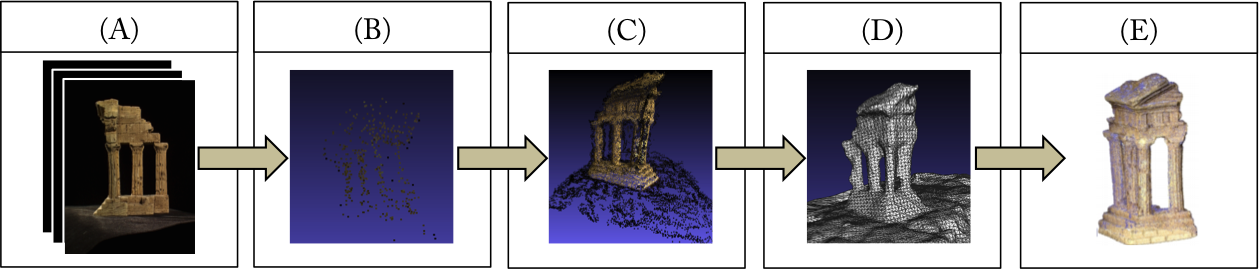
\includegraphics[width=\linewidth]{pipeline3.png}
  \end{center}
  \caption{Proposed Multi-View pipeline. (A) Source Images with known camera parameters. (B) Bundler Adjustment that utilizes feature matching to create a sparse point cloud. (C) Dense Recontruction that performs clustering to develop a more compact point cloud. (D) Surface Reconstruction adds a mesh to the points. (E) Applying colored textures on the mesh results in a realistic simulated model.}
  \label{fig:short}
\end{figure*}

\subsubsection{Point Based Approaches}

Once we have calibrated cameras with a sparse reconstruction, we can search along equipolar lines to find more correspondence points. The real-world locations of these points can be found through triangulation. In Patch-based Multi-View Stereo, these points were further expanded to \emph{patches} which included a color and normal vector.\cite{furukawa}

\subsubsection{Volumetric Approaches}

Another approach to dense reconstruction is to start with a volume which encloses the region of interest, and iteratively remove small sections (\emph{voxels}) which are not photoconsistent. Constructing the initial visual hull requires segmenting the input images into foreground and background.\cite{spacecarving}

\subsubsection{Stereo Depth Approaches}

A final approach is to build off research in stereo matching. Here, we generate depth maps for all pairs of images with overlapping fields of views. Methods include SemiGlobal Matching, Graph Cuts, and Dynamic Programming.\cite{sgm,taxonomy} These depth maps can be fused to extract the structure of the scene.\cite{fuse}

% \subsection{Surface Reconstruction}
% Mesh fitting
% Poisson Surface reconstruction
% Iterative Snapping [Furukawa]
% Marching Squares/Tetrahedrons
% Voronoi

\section{Surface Reconstruction}
We next want to reconstruct the surface given a finite set of scattered points.  This can be viewed as an optimization problem in which the overall goal is to minimize a global \textit{energy} function characterized by the constraints of the point cloud. \cite{mesh_opt}  Two common approaches to solve this problem include (1) interpolating the points with computational geometry and (2) constructing implicit functions to fit the data.

\subsection{ Geometric Estimation }
In this approach, the point cloud is partitioned into sections and geometric estimations are calculated at each point. For example, each point can be treated as a tangent plane and neighboring points are then projected onto this plane, giving an estimation of the surface point.\cite{surface_review, hoppe1992surface}  This utilizes methods such as Delanunay triangles, $\alpha$-shapes. \cite{surface_review, poisson} 

\subsection{ Function Fitting}
A more rigorous approach is to fit implicit (inside-outside) functions onto the point cloud.  This can be based on signed distance or centered radial basis functions (RBFs).\cite{poisson}  Improvements can be made to handle irregularities and outliers with the use of Moving Least Squares (MLS).\cite{szeliski2010computer}  Finding a continuous function in which the points approximately lie on the zero set determines the boundary for the mesh.  One way this can be completed is by the Marching Cubes Algorithm.\cite{hoppe1992surface}

As an example, \textit{Poisson Surface Reconstruction} utilizes the function fitting approach.  An inside-outside function is defined by gradients determined from the point normals.\cite{poisson}  In general, when undergoing surface reconstruction, it is important to ensure photoconsistencey is maintained. 

% Mesh fitting
% Poisson Surface reconstruction
% Iterative Snapping [Furukawa]
% Marching Squares/Tetrahedrons
% Voronoi

\section{Our Approach}

We will construct a pipeline which uses point-based methods to develop a densely reconstructed point cloud. From there, we will compare various mesh-fitting surface techniques.  We plan to compare the results quantitatively evaluate them qualitatively, using the Oculus Rift.  Figure 1 summarizes the overall reconstruction process.

\subsection{Visualization}
With a 3D reconstruction, it makes sense to try to view it in three dimensions. We do this using the Oculus Rift, a head-mounted stereoscopic display. We will render the scene in a game engine \cite{unity}, which will allow users to move around the scene.

\subsection{Conclusion}
There are many applications and approaches to Multi-View Stereo. We propose a pipeline which transforms a set of images into a model of the scene.  Additionally, we propose to visualize our results using an Oculus Rift, which will shed light on the reconstruction process.


% WE NEED TO ADD OUR SOURCES

{\small
  \bibliographystyle{ieee}
  \bibliography{egbib}
}

\end{document}
